\subsection{Adquisici�n}
\begin{frame}
\frametitle{}

\begin{figure}
\begin{tikzpicture}[node distance=0.5cm, auto,>=latex', thick]
\scriptsize
    % We need to set at bounding box first. Otherwise the diagram
    % will change position for each frame.
    \path[use as bounding box] (-1.5,0) rectangle (12,-2);

    % TT methodology     
    \node [phase]                        (monitoreo)     {Vigilancia};
    \node [phase, below of=monitoreo]    (choice)        {Elecci�n};
    \node [phase2,below of=choice]       (acquisition)   {Adquisici�n};
    \node [phase, below of=acquisition]  (adaptation)    {Adaptaci�n};
    \node [phase, below of=adaptation]   (absortion)     {Absorci�n};
    \node [phase, below of=absortion]    (aplication)    {Aplicaci�n};
    \node [phase, below of=aplication]   (difusion)      {Difusi�n};

    %%%%%%%%%%%%%%%%%%%%%%%%%%%%%%%%%%%%%%%%%%%%&
    %            Adquisici�n
    %%%%%%%%%%%%%%%%%%%%%%%%%%%%%%%%%%%%%%%%%%%%&
    \onslide<1> \node [ph_explain, right=.5cm of adaptation.east] (exp_acquisition)   
    {      
     \begin{center} \textbf{Adquisici�n} \end{center}
     \begin{itemize}
      \item Adquisici�n de equipos que utilicen la tecnolog�a que se desea transferir.
      \item F�cil adquisici�n.
        \begin{itemize}
        \scriptsize
         \item Existen aplicaciones en gran parte de las actividades humanas.
         \item No es necesario firmar acuerdos con pa�ses o con grandes industrias.
        \end{itemize}
      \item Adquisici�n de plataformas de desarrollo hardware y software 
      \item Identificaci�n de herramientas de desarrollo.
     \end{itemize}
    };


    \onslide<2> \node [ph_explain, right=.5cm of adaptation.east] (exp_acquisition)   
    {      
     \begin{center} \textbf{Adquisici�n} \end{center}
      \begin{center} 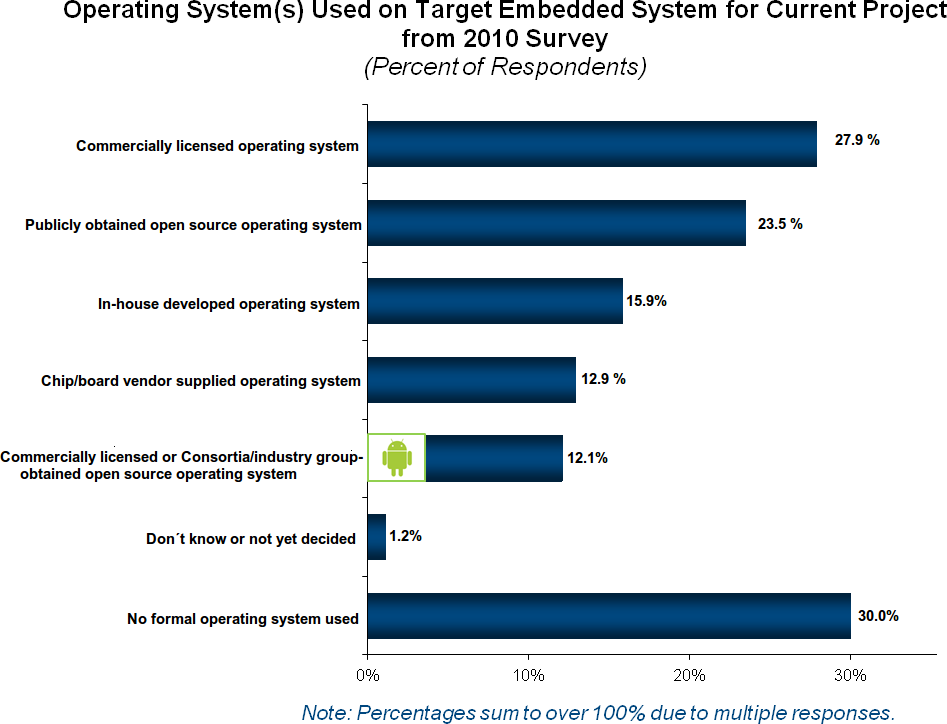
\includegraphics[scale=.45]{../images/embedded_os_trends.png} \end{center}
      \caption{\footnotesize Comparaci�n del uso de sistemas operativos Fuente: Venture Development Corp} \label{os_trends}
    };

    \onslide<3> \node [ph_explain, right=.5cm of adaptation.east] (exp_acquisition)   
    {      
     \begin{center} \textbf{Adquisici�n} \end{center}
      \begin{center} 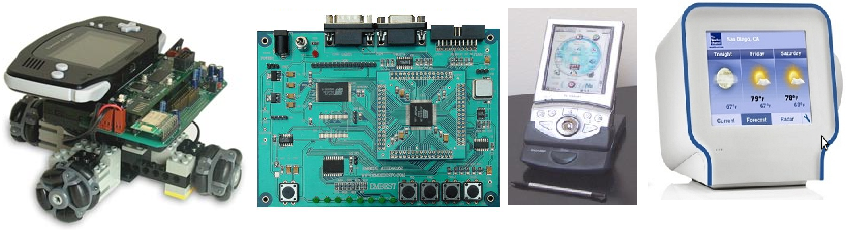
\includegraphics[scale=.3]{../images/plataformas_adquiridas.png} \\
        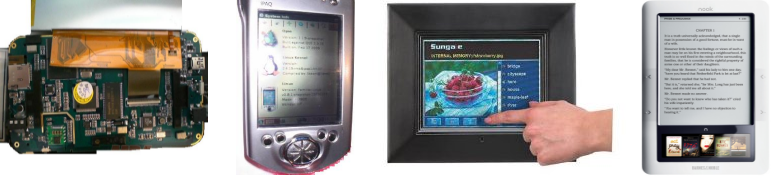
\includegraphics[scale=.29]{../images/plataformas_adquiridas2.png}
      \end{center}
      \caption{Plataformas adquiridas para el estudio de los sistemas emebebidos} 
    };
    
\end{tikzpicture}
\end{figure}

\end{frame}